\documentclass{standalone}
\usepackage{tikz}
\usetikzlibrary{angles,quotes}
\begin{document}
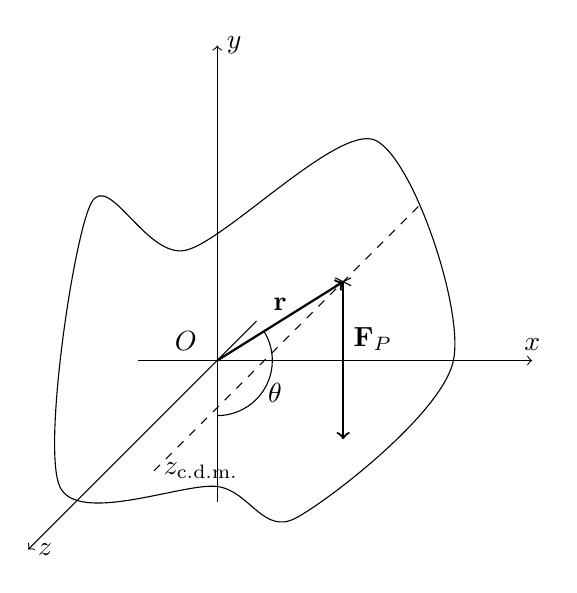
\begin{tikzpicture}[scale=2]
    \coordinate(O)at(0,0);
    \draw[->](-0.5,0)--(2,0)node[above]{$x$};
    \draw[->](0,-0.5)--(0,2)coordinate(z)node[right]{$y$};
    \draw[->](0.25,0.25)--(-1.2,-1.2)node[right]{$z$}; 
    \node[above]at(-0.2,0){$O$};
    
    \coordinate(cdm)at(0.8,0.5);
    
    \draw[-](0.75,0.475)--(0.85,0.525);
    \draw[-](0.75,0.525)--(0.85,0.475);
    \draw[-](O)--(0,-0.9)coordinate(y);
    \draw[thick, ->](cdm)--(0.8,-0.5)node[midway, above right]{$\mathbf{F}_P$};

    \draw[thick, ->](O)--(cdm)node[midway, above]{$\mathbf{r}$};

    \draw[dashed](-0.4,-0.7)node[right]{$z_{\mathrm{c.d.m.}}$}--(1.3,1);

    \draw[-]plot[smooth cycle]coordinates{(1.5,0)(1,1.4)(-0.2,0.7)(-0.8,1)(-1,-0.8)(0,-0.8)(0.5,-1)};
    \pic["$\theta$",draw,angle eccentricity=1.2,angle radius=0.7cm]{angle=y--O--cdm};
\end{tikzpicture}
\end{document}